% !TeX root = ../sustechthesis-example.tex

\chapter{补充内容}

一些数学、图片、表格、代码等的补充... 

\begin{figure}
    \centering
    \caption[8位超前进位加法器的FPGA实现结构图]{8位超前进位加法器的FPGA实现结构图(Vivado)\label{fig:ahead_adder_8bits}}
    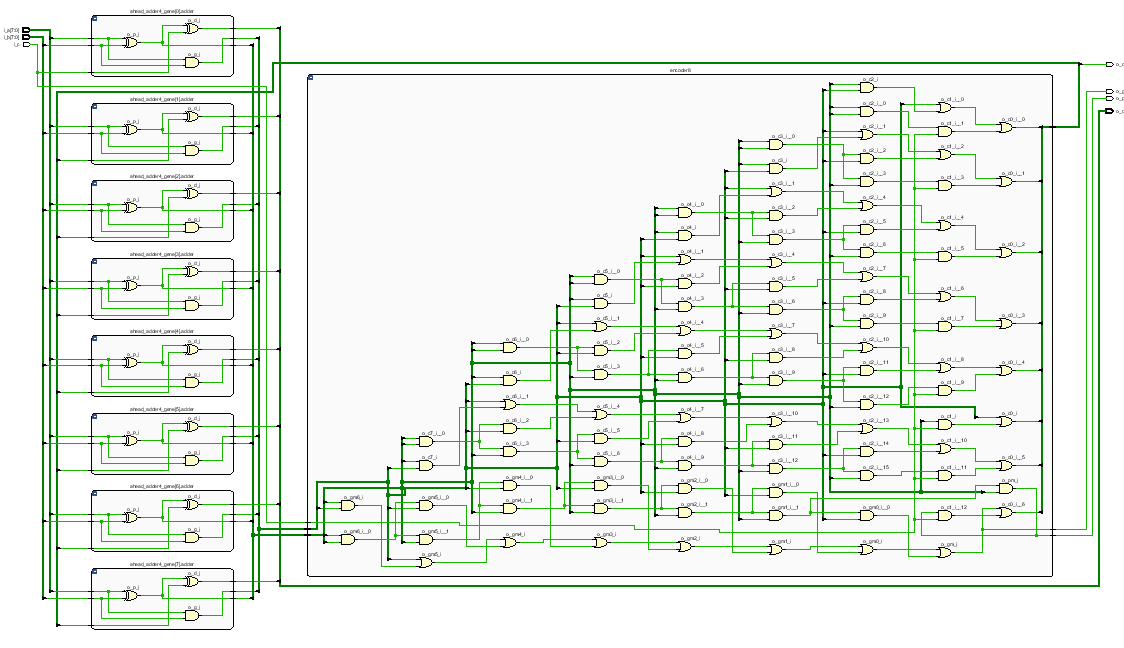
\includegraphics[width=1.0\linewidth]{rtmq/ahead_adder_8bits}
\end{figure}

\begin{figure}
    \centering
    \caption[16位超前进位加法器的FPGA实现结构图]{16位超前进位加法器的FPGA实现结构图(Vivado)\label{fig:ahead_adder_16bits}}
    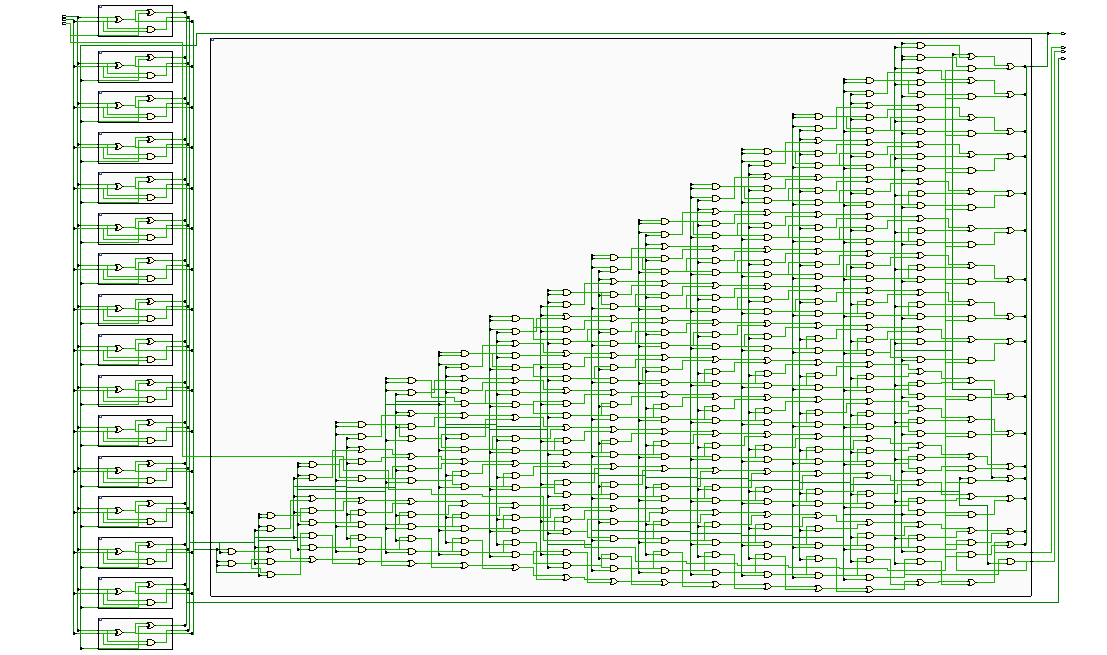
\includegraphics[width=1.0\linewidth]{rtmq/ahead_adder_16bits}
\end{figure}


\begin{figure}
    \centering
    \caption[32位Booth乘法器编码和加法树表]{32位Booth乘法器编码和加法树表\label{fig:booth_multiplier_32bits_basic}}
    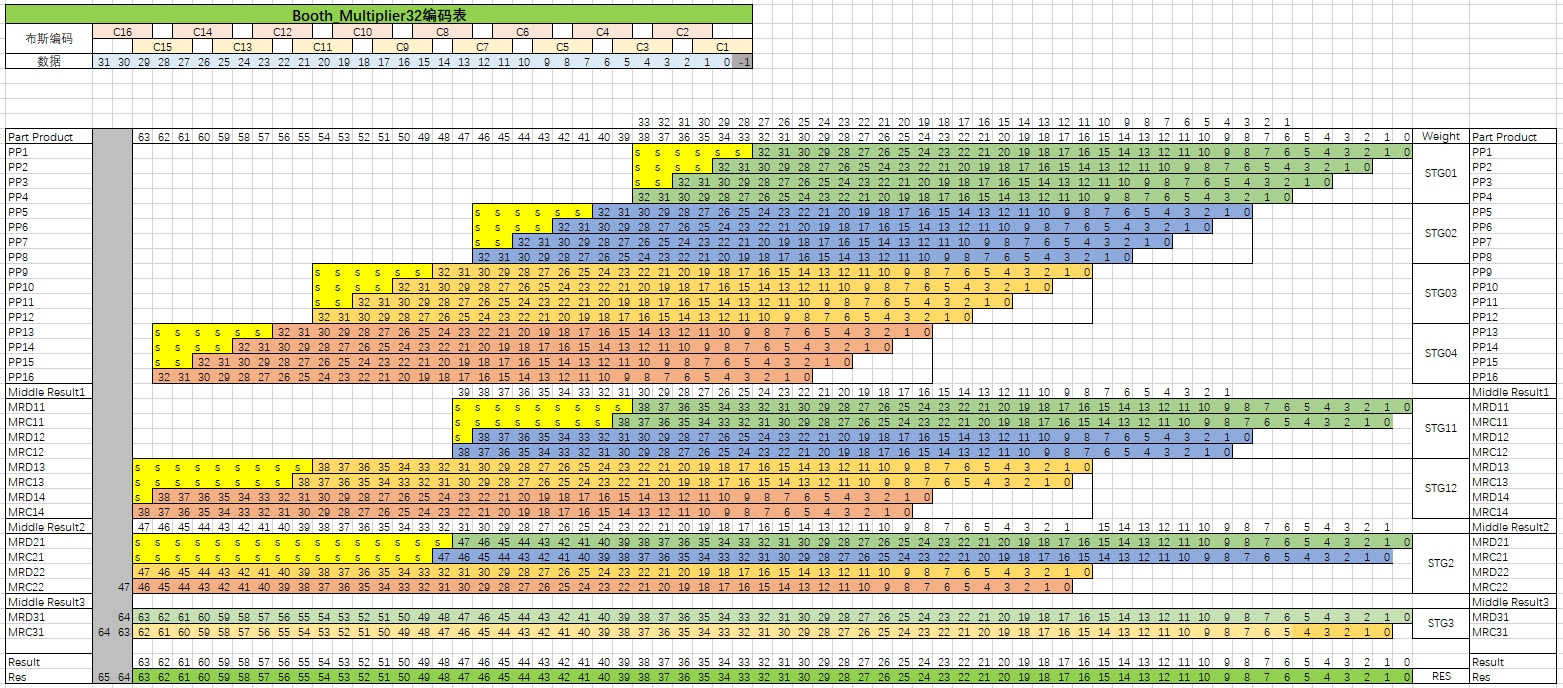
\includegraphics[width=1.0\linewidth]{rtmq/booth_multiplier_32bits_basic}
\end{figure}
